\chapter{Mengenal Kecerdasan Buatan dan Scikit-Learn}
\section{Teori}
Definisi, Sejarah, \& Perkembangan Kecerdasan Buatan
\begin{enumerate}
    \item Definisi
    Artificial Intelligence adalah sistem kecerdasan yang ditanamkan atau ditambahkan oleh manusia ke dalam suatu teknologi, yang nantinya akan dikembangkan dalam konteks ilmiah atau bentukan dari entitas ilmiah yang sudah ada.
    \item Sejarah
    Bermula dari kemunculan komputer sekitar th 1940-an, McMulloh dan Pitts pada tahun 1943 mengusulkan model matematis bernama perceptron dari neuron di dalam  otak. hal ini bagaimana neuron menjadi aktif seperti saklar on-off dan neuron tersebut mampu untuk belajar dan memberikan aksi berbeda terhadap waktu dari input yang diberikan.\\ 
    Sumbangan terbesar di bidang AI diawali pada paper Alan Turing di tahun 1950 untuk tahap riset awal proyek AI, tujuannya yaitu mengeksplorasi topik penyelesaian masalah dan metode simbolik.
    \item Perkembangan AI dimulai Pada tahun 1960 -an, Departemen Pertahanan dari Amerika Serikat juga mempunyai keinginan untuk mengembangkan dan melatih komputer agar memiliki penalaran seperti manusia secara mendasar. Sekitar tahun 1970 -an, proyek DARPA (Defence Advanced Research Project Agency) berhasil menyelesaikan studi kasus mengenai pemetaan jalan. Dan di awal abad ke – 21, tepatnya pada tahun 2003, DARPA juga sukses untuk menghasilkan asisten pribadi cerdas. Setelah itu, teknologi AI terus mengalami perkembangan hingga saat ini masuk pada program yang lebih detail lagi, dengan menerapkan algoritma dari deep learning (pembelajaran secara mendalam). Dimana, kecerdasan buatan yang dikembangkan mampu untuk mengerjakan tugas dan memberikan solusi secara lebih kompleks dengan kondisi yang lebih bervariatif.
\end{enumerate}
Definisi supervised learning, klasifikasi, regresi dan unsupervised learning. Data set, training set dan testing set.
\begin{enumerate}
    \item Supervised learning adalah algoritma yang paling sering digunakan dalam dunia data science. yang digunakan dalam memprediksi pola dimana pola tersebut sudah ada contoh data yang lengkap, maka pola yang terbentuk adalah hasil pembelajaran data lengkap tersebut.
    \item Klasifikasi adalah pengelompokkan sesuatu berdasarkan kelas-kelasnya, persamaan ciri dan perbedaannya.
    \item Regresi adalah salah satu metode untuk menentukan hubungan sebab-akibat antara variabel dengan variabel lainnya. selain itu ialah metode analisis yang digunakan dalam statistika, yang juga berguna untuk melihat pengaruh antara dua variabel atau lebih.
    \item Unsupervised learning adalah salah satu tipe algoritma machine learning yang digunakan untuk menarik kesimpulan dari dataset. Sehingga metode unsupervised learning yang paling umum adalah analisis cluster, yang digunakan pada analisa data untuk mencari pola-pola tersembunyi atau pengelompokan dalam data.
    \item Data set adalah sebuah himpunan data yang berasal dari informasi kumpulan data yang akan diinputkan dan diproses, dapat berupa record, point, vector, pattern, observation, case, dll, pada masa-masa lampau dan dikelola menjadi sebuah informasi untuk melakukan teknik dari ilmu data mining.
    \item Training set adalah bagian dataset yang kita latih untuk membuat prediksi atau klasifikasi untuk menjalankan fungsi dari sebuah algoritma ML.
    \item Testing set merupakan bagian dari data set yang digunakan untuk mengukur sejauh mana classifier berhasil melakukan klasifikasi dengan benar.
\end{enumerate}

\section{Instalasi}
\begin{enumerate}
    \item Instalasi library scikit Berikut ini merupakan tutorial cara menginstalasi library scikit dari Anaconda, mencoba kompilasi dan uji coba ambil contoh kode dan lihat variabel explorer.
    
	\begin{figure}
	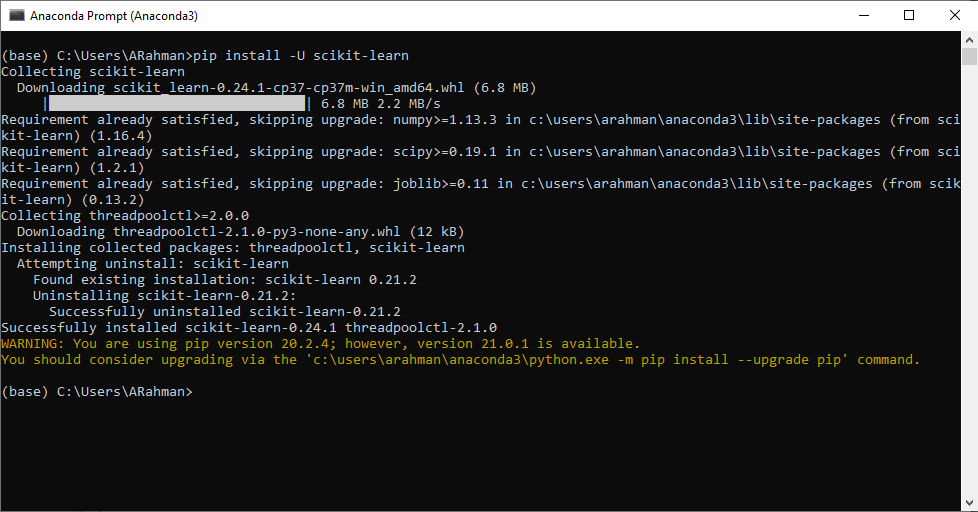
\includegraphics[scale=0.5]{section/ai2.png}
	\centering
	\caption{Instalasi Library Scikit-Learn}
	\end{figure}
	
	\begin{figure}
	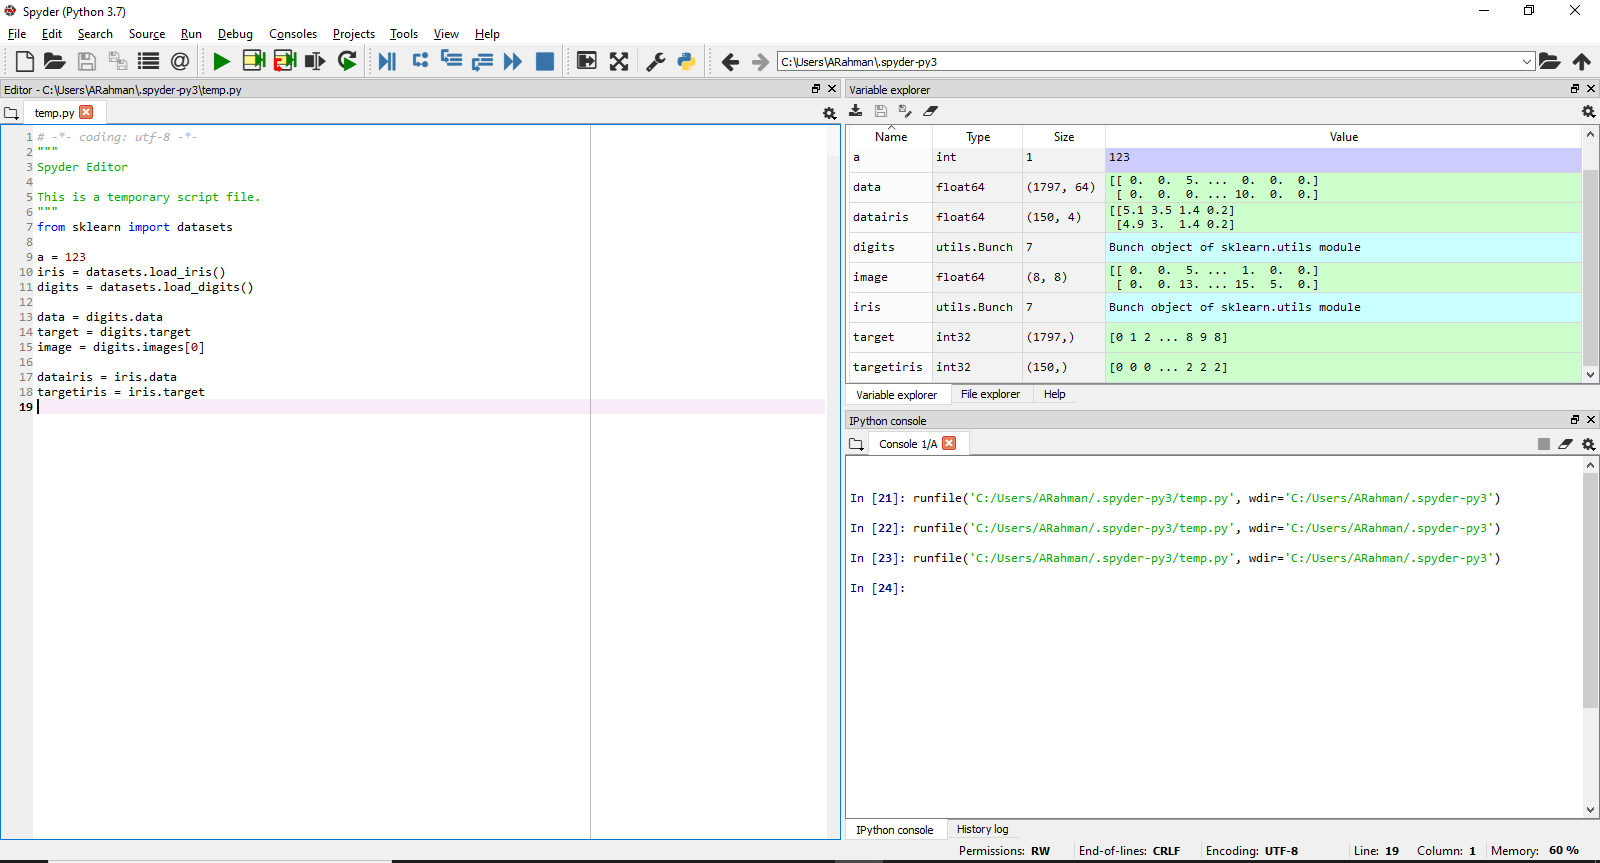
\includegraphics[scale=0.38]{section/ai3.png}
	\centering
	\caption{Variable Explorer}
	\end{figure}
	
\end{enumerate}